\documentclass[
11pt, % The default document font size, options: 10pt, 11pt, 12pt
%codirector, % Uncomment to add a codirector to the title page
]{charter} 


% El títulos de la memoria, se usa en la carátula y se puede usar el cualquier lugar del documento con el comando \ttitle
\titulo{Diseño e implementación de motor de afinidad para personalización comercial B2B en consumo masivo} 

% Nombre del posgrado, se usa en la carátula y se puede usar el cualquier lugar del documento con el comando \degreename
\posgrado{Carrera de Especialización en Inteligencia Artificial}

% Tu nombre, se puede usar el cualquier lugar del documento con el comando \authorname
\autor{Lic. Abril Noguera}

% El nombre del director y co-director, se puede usar el cualquier lugar del documento con el comando \supname y \cosupname y \pertesupname y \pertecosupname
\director{Ing. Juan Pablo Rodríguez Varela}
\pertenenciaDirector{ITBA} 
\codirector{} % para que aparezca en la portada se debe descomentar la opción codirector en los parámetros de documentclass
\pertenenciaCoDirector{FIUBA}

% Nombre del cliente, quien va a aprobar los resultados del proyecto, se puede usar con el comando \clientename y \empclientename
\cliente{MSc. Lautaro Gonzalez}
\empresaCliente{Empresa Líder de Consumo Masivo}
 
\fechaINICIO{01 de mayo de 2025}		%Fecha de inicio de la cursada de GdP \fechaInicioName
\fechaFINALPlan{17 de junio de 2025} 	%Fecha de final de cursada de GdP
\fechaFINALTrabajo{19 de diciembre de 2025}	%Fecha de defensa pública del trabajo final

% Agrego paquetes
\usepackage{pgfgantt}
\usepackage{datetime2}
\usepackage{xcolor}

\begin{document}

\maketitle
\thispagestyle{empty}
\pagebreak


\thispagestyle{empty}
{\setlength{\parskip}{0pt}
\tableofcontents{}
}
\pagebreak


\section*{Registros de cambios}
\label{sec:registro}


\begin{table}[ht]
\label{tab:registro}
\centering
\begin{tabularx}{\linewidth}{@{}|c|X|c|@{}}
\hline
\rowcolor[HTML]{C0C0C0} 
Revisión & \multicolumn{1}{c|}{\cellcolor[HTML]{C0C0C0}Detalles de los cambios realizados} & Fecha      \\ \hline
0      & Creación del documento                                 &\fechaInicioName \\ \hline
1      & Se completa hasta el punto 5 inclusive                & 13 de mayo de 2025 \\ \hline
2      & Se completa hasta el punto 9 inclusive                 & 20 de mayo de 2025 \\ \hline
3      & Se completa hasta el punto 12 inclusive                & 27 de mayo de 2025 \\ \hline
4      & Se completa el plan	                                 & 3 de junio de 2025 \\ \hline

% Si hay más correcciones pasada la versión 4 también se deben especificar acá

\end{tabularx}
\end{table}

\pagebreak

\section*{Acta de constitución del proyecto}
\label{sec:acta}

\begin{flushright}
Buenos Aires, \fechaInicioName
\end{flushright}

\vspace{2cm}

%Presupuesto: Sueldo (Hora Hombre * 600hs) + Clusters + Compu = $ 13.500.000

Por medio de la presente se acuerda con la \authorname\hspace{1px} que su Trabajo Final de la \degreename\hspace{1px} se titulará ``\ttitle'' y consistirá en el desarrollo e integración de un sistema de recomendación que estime el interés potencial de cada cliente por los productos del portafolio de la empresa, a partir de señales de comportamiento en su canal digital de ventas. El trabajo tendrá un presupuesto preliminar estimado de 600 horas y un costo estimado de \$ 13.500.000, con fecha de inicio el \fechaInicioName\hspace{1px} y fecha de presentación pública el \fechaFinalName.

Se adjunta a esta acta la planificación inicial.

\vfill

% Esta parte se construye sola con la información que hayan cargado en el preámbulo del documento y no debe modificarla
\begin{table}[ht]
\centering
\begin{tabular}{ccc}
\begin{tabular}[c]{@{}c@{}}Dr. Ing. Ariel Lutenberg \\ Director posgrado FIUBA\end{tabular} & \hspace{2cm} & \begin{tabular}[c]{@{}c@{}}\clientename \\ \empclientename \end{tabular} \vspace{2.5cm} \\ 
\multicolumn{3}{c}{\begin{tabular}[c]{@{}c@{}} \supname \\ Director del trabajo final\end{tabular}} \vspace{2.5cm} \\
\end{tabular}
\end{table}




\section{1. Descripción técnica-conceptual del proyecto a realizar}
\label{sec:descripcion}

\subsection{Definición del Problema}

En el sector de consumo masivo, especialmente en modelos de negocio \textit{Business-to-Business (B2B)}, estimar el interés potencial entre clientes y productos desempeña un papel crucial en la optimización de estrategias comerciales.  Esta predicción se utiliza para priorizar qué productos sugerir a cada punto de venta en cada ciclo comercial, permitiendo adaptar las recomendaciones a las preferencias y comportamientos reales de cada cliente. En lugar de ofrecer el mismo conjunto de productos a todos los clientes o basarse únicamente en el historial de compra, contar con una calificación de afinidad posibilita ordenar el portafolio según relevancia, potenciar la venta cruzada y mejorar la eficiencia en el uso del canal digital. Además, brinda al equipo comercial una herramienta concreta para planificar visitas, personalizar ofertas y detectar oportunidades antes no visibles, especialmente en productos nuevos o categorías estratégicas.

La naturaleza del negocio B2B trae más complejidad. A diferencia de los consumidores finales, cuyos patrones de compra suelen ser más regulares y predecibles, los minoristas ajustan sus pedidos en función de variables como la estacionalidad, las promociones comerciales y el comportamiento fluctuante de sus propios clientes. Esta variabilidad se acentúa cuando analizamos la marcada diversidad entre los distintos puntos de venta: desde pequeños kioscos urbanos con espacio limitado para exhibición hasta grandes supermercados con capacidad para gestionar amplios surtidos. Cada uno presenta necesidades y capacidades logísticas radicalmente diferentes.

Además, la constante rotación e incorporación de nuevos productos en el portafolio genera un escenario de permanente adaptación. En la práctica se observa que aproximadamente el 12\% del catálogo se renueva anualmente. Este desafío es conocido como "\textit{cold start}", la dificultad para recomendar productos sin historial transaccional. Este problema se vuelve aún más desafiante porque, incluso entre los productos que ya tienen historial de ventas, muchos presentan compras muy esporádicas o aisladas. Esto genera un conjunto de datos con poca información por producto, lo que dificulta que los modelos tradicionales puedan aprender patrones consistentes para hacer buenas recomendaciones.

El ecosistema B2B presenta particularidades que exigen soluciones a medida. Estas deben ir más allá de los enfoques tradicionales de recomendación para incorporar, además de datos transaccionales históricos, información contextual sobre los puntos de venta, señales de comportamiento digital e inteligencia de negocio que permitan capturar las particularidades de cada relación comercial. El desarrollo de este tipo de sistemas permite calcular un \textit{score} de afinidad entre cada cliente y cada producto del portafolio. Esto refleja qué tan relevante podría ser ese ítem para ese punto de venta en un momento determinado. Estas puntuaciones pueden luego ser ordenadas para generar \textit{rankings} personalizados que sirvan como insumo para la toma de decisiones comerciales y habilita una estrategia más proactiva y adaptada al comportamiento real de cada cliente.

\subsection{Descripción Funcional}

La solución se organiza en distintos módulos que trabajan de manera integrada para calcular y actualizar, de forma periódica, un nivel de afinidad entre cada cliente y cada producto. El sistema opera de forma cíclica y está compuesto por cinco bloques funcionales que reflejan las etapas clave del proceso. En la figura \ref{fig:diagBloques} se presenta el diagrama en bloques del sistema. 

\begin{figure}[htpb]
\centering 
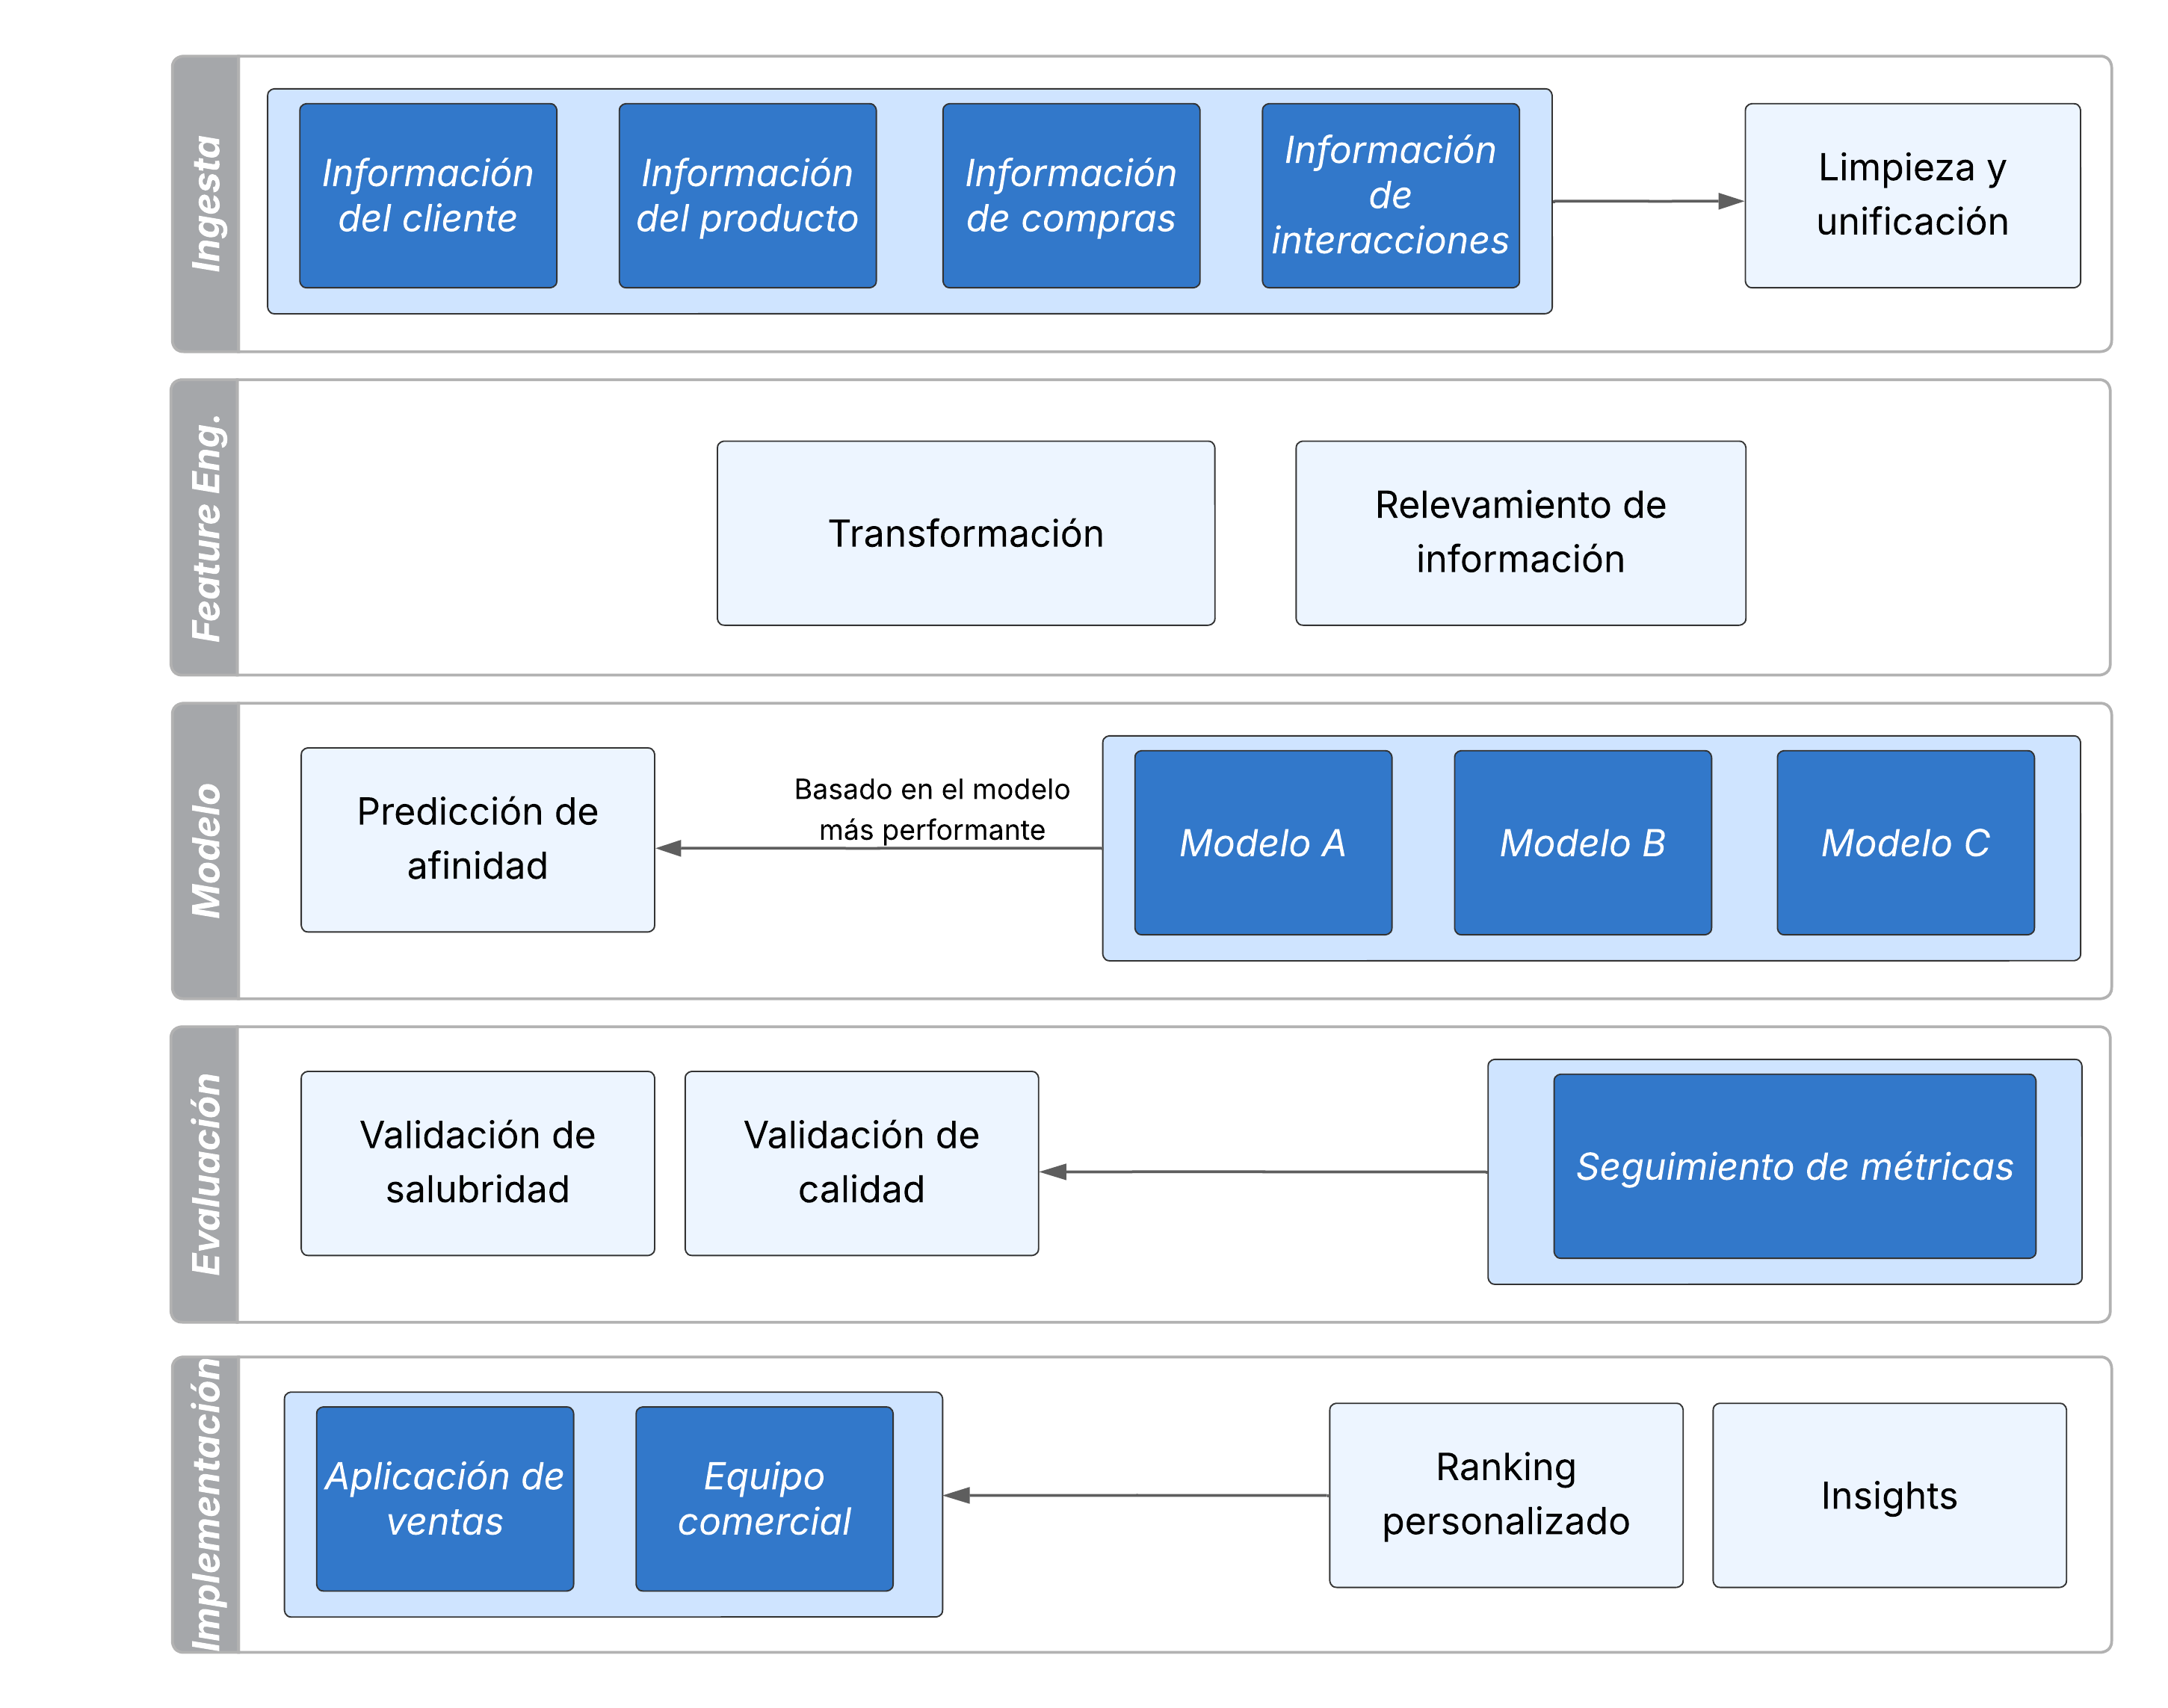
\includegraphics[width=.85\textwidth]{./Figuras/diagBloques.png}
\caption{Diagrama en bloques del sistema.}
\label{fig:diagBloques}
\end{figure}

En primer lugar, se realiza la ingesta y consolidación de la información necesaria para alimentar el modelo. El sistema combina distintas fuentes internas con el objetivo de comprender en profundidad las preferencias de cada punto de venta. Por una parte, se analiza el historial de compras para identificar los productos que han resultado más relevantes según el tipo de negocio. Por otra, se incorpora el registro de interacciones digitales, como búsquedas, visualizaciones y agregados al carrito que no derivaron en una compra. Esta información se completa con características del cliente, como la ubicación, el tamaño del establecimiento y el perfil del consumidor final, junto con atributos del producto, como la categoría, la marca y su posición dentro del portafolio. El objetivo de esta etapa es construir una base robusta que permita representar de manera integral la relación entre clientes y productos.

A continuación, los datos procesados se convierten en variables que resumen el comportamiento del cliente frente a cada producto. Estas variables incluyen la frecuencia y la recencia de las interacciones, la variedad de categorías exploradas y la intensidad de actividad en distintos períodos. También se incorporan indicadores contextuales, como la popularidad del producto en grupos de clientes similares o el nivel de exposición previa. Este conjunto de variables constituye la entrada del modelo que calcula el valor de afinidad entre cada cliente y cada producto.

El valor estimado representa una medida continua que refleja la relevancia potencial de un producto para un punto de venta específico. Esta puntuación permite ordenar los productos según su grado de interés relativo y se actualiza de forma periódica para adaptarse a los cambios en el comportamiento comercial. El modelo utilizado será seleccionado en función de su desempeño, comparando diferentes alternativas con base en las métricas definidas.

Una vez calculadas las puntuaciones, se evalúa la calidad de las recomendaciones a través de métricas específicas del ámbito de los sistemas de recomendación. Entre las más relevantes se encuentran el \textit{recall} en el top K, la cobertura del portafolio, la diversidad de las sugerencias generadas y la precisión media promedio. Estas métricas permiten monitorear el desempeño general del sistema y detectar oportunidades de mejora tanto a nivel global como por segmento de cliente.

Finalmente, los resultados se integran en los procesos comerciales existentes mediante listas priorizadas de productos para cada cliente. Estas recomendaciones pueden ser visualizadas en la aplicación de ventas o utilizadas por el equipo comercial como herramienta de planificación. De esta forma, el sistema aporta valor concreto al negocio al facilitar sugerencias más relevantes, alineadas con el comportamiento observado y consistentes con los objetivos comerciales de la compañía.

\section{2. Identificación y análisis de los interesados}
\label{sec:interesados}

El proyecto involucra a distintos actores relevantes en su desarrollo, validación y futura aplicación.  El cliente, quien se desempeña como Director del equipo de Data en la \empclientename, es el principal impulsor de la iniciativa y sponsor del proyecto. En particular, se destaca la participación del equipo de Portfolio Strategy como usuario final del sistema, representado por su Product Owner (PO), quien actúa como principal referente funcional y articula entre los requerimientos del negocio y las decisiones técnicas. La responsable directa del desarrollo es la autora de este trabajo, quien llevará adelante el diseño, desarrollo y la implementación de la solución. La siguiente tabla resume estos roles y sus respectivas organizaciones.

\begin{table}[ht]
%\caption{Identificación de los interesados}
%\label{tab:interesados}
\begin{tabularx}{\linewidth}{@{}|l|X|X|l|@{}}
\hline
\rowcolor[HTML]{C0C0C0} 
Rol           & Nombre y Apellido & Organización 	& Puesto 	\\ \hline
% Auspiciante   &                   &              	&        	\\ \hline
Cliente       & \clientename      &\empclientename	& Gerente del proyecto       	\\ \hline
% Impulsor      &                   &              	&        	\\ \hline
Responsable   & \authorname       & FIUBA        	& Alumno 	\\ \hline
%Colaboradores &                   &              	&        	\\ \hline
Orientador    & \supname	      & \pertesupname 	& Director del trabajo final \\ \hline
% Equipo        & miembro1 \newline 
%				miembro2          &              	&        	\\ \hline
% Opositores    &                   &              	&        	\\ \hline
Usuario final &  Lic. Micaela Bassan    & \empclientename	&  \textit{Product owner} \\ \hline
\end{tabularx}
\end{table}

\section{3. Propósito del proyecto}
\label{sec:proposito}

El propósito del proyecto es desarrollar un sistema que estime la relevancia potencial de cada producto para cada punto de venta, a partir de información transaccional, comportamientos digitales y atributos contextuales.  Esta estimación permitirá generar listas personalizadas que orienten la planificación comercial y sirvan como insumo para la toma de decisiones. Se busca mejorar la precisión de las sugerencias, ampliar la visibilidad de productos estratégicos y avanzar hacia una gestión más proactiva, escalable y basada en datos, alineada con los objetivos comerciales de la compañía.

\section{4. Alcance del proyecto}
\label{sec:alcance}

El universo sobre el que se desarrollará esta iniciativa corresponde al conjunto de clientes y productos gestionado por el equipo de Portfolio Strategy en Argentina. Este se limita a clientes activos pertenecientes a los canales de Kioscos, tradicionales y autoservicios, bajo el régimen \textit{off premise}\footnote{Off premise refiere a puntos de venta donde el producto es adquirido para consumo fuera del establecimiento.}. La cartera de productos considerada se enfoca exclusivamente en bebidas. Quedan excluidos del alcance los clientes de los canales \textit{on premise}, supermercados y mayoristas, dado que presentan dinámicas comerciales significativamente diferentes y representan una fracción menor del total. Tampoco se contempla el negocio de marketplace, debido a sus particularidades operativas y a su peso relativamente reducido dentro del universo analizado.

El desarrollo del proyecto se organiza en una serie de etapas que abarcan desde la exploración inicial del estado del arte hasta la implementación del modelo y su evaluación en entorno real. Estas etapas permiten avanzar de forma iterativa y asegurar la calidad del entregable final, tanto desde el punto de vista técnico como funcional. A continuación, se detallan las principales actividades previstas:

\begin{itemize}
\item Relevamiento de modelos \textit{benchmark} y revisión del estado del arte.
\item Definición de métricas de éxito del proyecto.
\item Desarrollo de un modelo \textit{baseline} como punto de comparación inicial.
\item Formulación de hipótesis orientadoras del enfoque propuesto.
\item Desarrollo del proceso de \textit{feature engineering}.
\item Entrenamiento y validación de modelos.
\item Evaluación de resultados con métricas de recomendación.
\item Construcción del pipeline de implementación.
\item Ejecución de pruebas tipo A/B.
\item Reporte y presentación de resultados.
\item Registro y disponibilización del modelo final en MLflow.
\end{itemize}

Si bien este desarrollo se enmarca en un universo específico de clientes y productos, el enfoque está diseñado de manera modular, con el objetivo de facilitar su adaptación a otros segmentos del negocio en caso de resultar exitoso.

\section{5. Supuestos del proyecto}
\label{sec:supuestos}

Para el desarrollo del presente proyecto se supone que: 
\begin{itemize}
	\item Se cuenta con acceso a las fuentes de información necesarias para el desarrollo de la solución. 
        \item No se producirán cambios significativos en los procesos comerciales o en la estructura de los datos durante el período de desarrollo.
	\item Se dispone con los accesos a recursos cloud y software necesarios para el desarrollo de la solución. 
	\item El tiempo asignado para completar el proyecto será suficiente.
        \item Los colaboradores e interesados clave disponen del tiempo para reuniones de validación y toma de decisiones.
\end{itemize}

\section{6. Product Backlog}
\label{sec:backlog}

La siguiente sección presenta el Product Backlog del proyecto, estructurado en torno a cuatro épicas principales que agrupan las funcionalidades clave del desarrollo. Cada épica contiene historias de usuario redactadas de forma concisa, con el objetivo de representar las necesidades del sistema desde la perspectiva de los distintos roles involucrados. Las historias incluyen su prioridad relativa, una estimación en Story Points y una breve descripción del propósito funcional. La asignación de Story Points se basa en una evaluación multidimensional que considera dificultad, complejidad e incertidumbre, y el valor total se redondea al número superior más próximo dentro de la secuencia de Fibonacci. Este enfoque busca facilitar la planificación de los sprintse y asegurar la trazabilidad entre objetivos, funcionalidades y entregables.

\subsection*{\'Epica 1: \textit{discovery} y entendimiento del problema}
\begin{itemize}
  \item \textbf{Historia 1:} como responsable del proyecto, quiero relevar y documentar las expectativas del cliente para alinear el desarrollo con sus objetivos.\\
  \textbf{Prioridad:} alta, \textbf{Story Points:} 5, \textbf{Justificación:} D:2, C:1, I:2 $\Rightarrow$ Total: 5

  \item \textbf{Historia 2:} como analista, quiero revisar el estado del arte para incorporar enfoques relevantes y detectar oportunidades.\\
  \textbf{Prioridad:} media, \textbf{Story Points:} 8, \textbf{Justificación:} D:2, C:2, I:3 $\Rightarrow$ Total: 7

  \item \textbf{Historia 3:} como responsable del proyecto, quiero definir KPIs y métricas para medir el desempeño de la solución.\\
  \textbf{Prioridad:} alta, \textbf{Story Points:} 5, \textbf{Justificación:} D:2, C:1, I:2 $\Rightarrow$ Total: 5
\end{itemize}

\subsection*{\'Epica 2: desarrollo de ingeniería de atributos}
\begin{itemize}
  \item \textbf{Historia 4:} como desarrolladora, quiero construir un proceso de extracción, transformación y carga (\textit{ETL}) que asegure calidad y consistencia en los datos.\\
  \textbf{Prioridad:} alta, \textbf{Story Points:} 8, \textbf{Justificación:} D:3, C:2, I:2 $\Rightarrow$ Total: 7

  \item \textbf{Historia 5:} como analista, quiero realizar un análisis exploratorio para entender patrones y relaciones en los datos.\\
  \textbf{Prioridad:} alta, \textbf{Story Points:} 5, \textbf{Justificación:} D:2, C:2, I:1 $\Rightarrow$ Total: 5

  \item \textbf{Historia 6:} como científica de datos, quiero construir variables relevantes para representar el comportamiento de clientes y productos.\\
  \textbf{Prioridad:} alta, \textbf{Story Points:} 8, \textbf{Justificación:} D:3, C:2, I:2 $\Rightarrow$ Total: 7
\end{itemize}

\subsection*{\'Epica 3: modelado y evaluación}
\begin{itemize}
  \item \textbf{Historia 7:} como responsable técnica, quiero desarrollar un modelo \textit{baseline} que sirva como comparación inicial.\\
  \textbf{Prioridad:} media, \textbf{Story Points:} 5, \textbf{Justificación:} D:2, C:2, I:1 $\Rightarrow$ Total: 5

  \item \textbf{Historia 8:} como científica de datos, quiero entrenar un modelo más avanzado para estimar afinidad con mayor precisión.\\
  \textbf{Prioridad:} alta, \textbf{Story Points:} 8, \textbf{Justificación:} D:3, C:2, I:3 $\Rightarrow$ Total: 8

  \item \textbf{Historia 9:} como equipo de proyecto, quiero evaluar el rendimiento del modelo con métricas apropiadas.\\
  \textbf{Prioridad:} alta, \textbf{Story Points:} 5, \textbf{Justificación:} D:2, C:1, I:2 $\Rightarrow$ Total: 5

  \item \textbf{Historia 10:} como desarrolladora, quiero registrar el modelo en MLflow para asegurar su trazabilidad.\\
  \textbf{Prioridad:} media, \textbf{Story Points:} 3, \textbf{Justificación:} D:1, C:1, I:1 $\Rightarrow$ Total: 3
\end{itemize}

\subsection*{\'Epica 4: implementación}
\begin{itemize}
  \item \textbf{Historia 11:} como responsable técnica, quiero preparar un \textit{pipeline} mensual que automatice la generación de \textit{scores}.\\
  \textbf{Prioridad:} alta, \textbf{Story Points:} 8, \textbf{Justificación:} D:3, C:2, I:3 $\Rightarrow$ Total: 8

  \item \textbf{Historia 12:} como analista de negocio, quiero ejecutar una prueba A/B para comparar el impacto del sistema.\\
  \textbf{Prioridad:} alta, \textbf{Story Points:} 8, \textbf{Justificación:} D:3, C:2, I:3 $\Rightarrow$ Total: 8

  \item \textbf{Historia 13:} como responsable del sistema, quiero monitorear el funcionamiento del modelo para asegurar su estabilidad.\\
  \textbf{Prioridad:} media, \textbf{Story Points:} 5, \textbf{Justificación:} D:2, C:2, I:1 $\Rightarrow$ Total: 5

  \item \textbf{Historia 14:} como responsable del proyecto, quiero presentar los resultados a los interesados para facilitar su adopción.\\
  \textbf{Prioridad:} alta, \textbf{Story Points:} 3, \textbf{Justificación:} D:1, C:1, I:1 $\Rightarrow$ Total: 3
\end{itemize}

\section{7. criterios de aceptación de historias de usuario}
\label{sec:criteriosAceptacion}

Los criterios de aceptación definen de forma objetiva cuándo una historia de usuario se considera completa y correctamente implementada. Están redactados de manera específica, medible y verificable, con el objetivo de validar que cada funcionalidad cumple con los requerimientos funcionales, técnicos y de presentación.

\textbf{\'Epica 1: \textit{discovery} y entendimiento del problema}
\begin{itemize}
  \item HU1: definir expectativas del cliente
  \begin{itemize}
    \item Se entrega un documento con los objetivos y necesidades del cliente validados por el sponsor.
    \item El documento se revisa en una reunión de validación.
  \end{itemize}
  \item HU2: analizar estado del arte
  \begin{itemize}
    \item Se entrega un informe con mínimo tres enfoques de referencia.
    \item El análisis incluye fortalezas y debilidades por enfoque.
    \item El PO valida la aplicabilidad a este caso.
  \end{itemize}
  \item HU3: definir métricas
  \begin{itemize}
    \item Se definen al menos tres métricas clave (recall, MAP, cobertura).
    \item Se documenta su forma de cálculo.
    \item Se aprueban en conjunto con el equipo técnico.
  \end{itemize}
\end{itemize}

\textbf{\'Epica 2: desarrollo de ingeniería de atributos}
\begin{itemize}
  \item HU4: construir proceso ETL
  \begin{itemize}
    \item El pipeline carga correctamente datos de todas las fuentes requeridas.
    \item El código pasa controles básicos de calidad.
    \item Se valida consistencia con una muestra aleatoria de registros.
  \end{itemize}
  \item HU5: realizar EDA
  \begin{itemize}
    \item Se entrega notebook con análisis descriptivo de las principales variables.
    \item Se identifican valores faltantes, atípicos y distribuciones.
    \item Los hallazgos se documentan y discuten en revisión técnica.
  \end{itemize}
  \item HU6: generar atributos
  \begin{itemize}
    \item Se construyen al menos 10 variables relevantes para el modelo.
    \item Se justifica cada atributo en función de comportamiento cliente-producto.
    \item Se validan estadísticas básicas y cobertura para cada \textit{feature}.
  \end{itemize}
\end{itemize}

\textbf{\'Epica 3: modelado y evaluación}
\begin{itemize}
  \item HU7: desarrollar modelo \textit{baseline}
  \begin{itemize}
    \item Se entrena un modelo sencillo como punto de referencia.
    \item El código está documentado y versionado.
    \item Se reportan las métricas definidas en la sección anterior.
  \end{itemize}
  \item HU8: desarrollar modelos \textit{benchmark}
  \begin{itemize}
    \item El modelo final obtiene mejora en al menos 2 métricas frente al \textit{baseline}.
    \item El pipeline de entrenamiento es reproducible.
    \item Se valida su comportamiento en distintos segmentos de cliente.
  \end{itemize}
  \item HU9: evaluación completa
  \begin{itemize}
    \item Se presentan los resultados completos por métrica y segmento.
    \item Se identifican debilidades del modelo y posibles mejoras.
    \item Se valida el cumplimiento de los objetivos del proyecto.
  \end{itemize}
  \item HU10: registro en MLflow
  \begin{itemize}
    \item El modelo se encuentra registrado con nombre, fecha, parámetros y métricas.
    \item Se puede reproducir y reutilizar desde el entorno técnico.
    \item Su versión queda asociada al entregable final.
  \end{itemize}
\end{itemize}

\textbf{\'Epica 4: implementación}
\begin{itemize}
  \item HU11: pipeline de producción
  \begin{itemize}
    \item El proceso mensual corre sin errores y genera resultados válidos.
    \item El output se integra al flujo operativo existente.
    \item Se documenta el proceso completo.
  \end{itemize}
  \item HU12: A/B testing
  \begin{itemize}
    \item Se define correctamente el grupo de control y tratamiento.
    \item Se mide el impacto de forma cuantitativa.
    \item El análisis es presentado con visualizaciones claras.
  \end{itemize}
  \item HU13: seguimiento de salubridad
  \begin{itemize}
    \item Se implementa un control automático de métricas clave.
    \item Se definen alertas en caso de desviaciones significativas.
    \item El equipo puede monitorear mensualmente los resultados.
  \end{itemize}
  \item HU14: presentación final
  \begin{itemize}
    \item Se elabora una presentación con objetivos, resultados y próximos pasos.
    \item Se presenta al equipo de datos y al PO.
    \item Se entrega junto con el entregable técnico final.
  \end{itemize}
\end{itemize}

\section{8. Fases de CRISP-DM}

El desarrollo del presente proyecto se estructura según la metodología CRISP-DM  \textit{(Cross Industry Standard Process for Data Mining)}, ampliamente utilizada en proyectos de ciencia de datos por su enfoque iterativo, modular y orientado al negocio. Esta metodología permite alinear los objetivos técnicos con las necesidades estratégicas, y organiza el trabajo en fases que van desde la comprensión del problema hasta la evaluación del modelo y su posterior implementación. A continuación, se detallan las principales etapas de CRISP-DM aplicadas a este caso.

\begin{enumerate}
\item \textbf{Comprensión del negocio:}
el objetivo del proyecto es desarrollar un sistema que permita estimar la relevancia potencial de cada producto para cada punto de venta, con el fin de generar \textit{rankings} personalizados que orienten las recomendaciones comerciales. El valor agregado de aplicar inteligencia artificial en este contexto radica en mejorar la precisión de las sugerencias, aumentar la cobertura del portafolio y optimizar la eficiencia del canal digital B2B. Las métricas de éxito incluyen recall@K, cobertura, MAP@K y diversidad de recomendaciones.

\item \textbf{Comprensión de los datos:}
los datos utilizados provienen de fuentes internas de la empresa e incluyen información transaccional, eventos digitales de la aplicación de ventas (visualizaciones, carritos, búsquedas) y atributos contextuales de productos y puntos de venta. La base de datos abarca clientes activos de los canales kioscos, tradicionales y autoservicios bajo régimen \textit{off Premise}, y se enfoca en productos del portafolio de bebidas. Se realizará un análisis exploratorio para evaluar la calidad, consistencia y completitud de los datos.

\item \textbf{Preparación de los datos:}
esta etapa incluye la construcción de un \textit{pipeline} de ETL que permita integrar y transformar los datos en una estructura analítica adecuada. Se generarán variables que capturen comportamiento histórico, exposición a productos, patrones de navegación y similitud con otros puntos de venta. La ingeniería de atributos buscará representar de manera compacta la relación cliente-producto con el objetivo de alimentar los modelos de predicción de afinidad.

\item \textbf{Modelado:}
se aborda un problema de recomendación basado en afinidad, con el uso de técnicas de aprendizaje supervisado y filtrado colaborativo, entre otras. Se exploran algoritmos como modelos de regresión regularizada, matrices de factorización y, en caso de que las alternativas más simples no alcancen el rendimiento esperado, se consideran modelos de \textit{ranking} o aprendizaje profundo.

\item \textbf{Evaluación del modelo:}
el desempeño de los modelos será evaluado mediante métricas propias del dominio de sistemas de recomendación, tales como recall@K, MAP@K, cobertura del portafolio sugerido y diversidad. La validación se realizará tanto de forma global como segmentada por tipo de cliente o categoría de producto. Los resultados serán comparados contra un modelo \textit{baseline} y validados junto al equipo funcional.

\item \textbf{Despliegue del modelo:}
en caso de ser validado, el modelo se integrará al sistema de recomendaciones mensuales de la empresa a través de un \textit{pipeline} automatizado. Los \textit{scores} generados se disponibilizarán en tablas de resultados que alimentan tanto la aplicación de ventas como las herramientas internas del equipo de Portfolio Strategy. El modelo será registrado y versionado en MLflow para facilitar su mantenimiento y evolución.
\end{enumerate}

\section{9. Desglose del trabajo en tareas}
\label{sec:wbs}

A partir de cada historia de usuario definida en el Product Backlog, se identifican tareas técnicas específicas y medibles. Estas tareas permiten una planificación más precisa del proyecto y constituyen la base para la definición de los sprints y del cronograma general. Las tareas están priorizadas según su impacto funcional y su necesidad para cumplir los criterios de aceptación asociados.

\begin{longtable}{|p{2cm}|p{9cm}|c|c|}
\hline
\rowcolor[HTML]{C0C0C0}
Historia de usuario & Tarea técnica & Estimación & Prioridad \\ \hline
\endfirsthead

\hline
\rowcolor[HTML]{C0C0C0}
Historia de usuario & Tarea técnica & Estimación & Prioridad \\ \hline
\endhead

HU1 & Levantar requerimientos con el sponsor. & 8 hs & Alta \\ \hline
HU1 & Documentar requerimientos del sponsor. & 8 hs & Alta \\ \hline

HU2 & Investigar al menos tres enfoques aplicados a problemas similares & 12 hs & Media \\ \hline
HU2 & Documentar enfoques \textit{benchmark} & 5 hs & Media \\ \hline

HU3 & Seleccionar métricas relevantes junto al equipo técnico & 9 hs & Alta \\ \hline
HU3 & Documentar métricas de seguimiento del proyecto  & 3 hs & Alta \\ \hline

HU4 & Diseñar pipeline de ingestión desde cada fuente de datos & 16 hs & Alta \\ \hline
HU4 & Implementar transformación de datos  & 12 h & Alta \\ \hline
HU4 & Testear integridad y consistencia de los datos ingresados & 12 hs & Alta \\ \hline

HU5 & Explorar variables clave: frecuencias, correlaciones, ,etc. & 8 hs & Alta \\ \hline
HU5 & Detectar y tratar valores extremos y nulos & 7 hs & Alta \\ \hline
HU5 & Presentar hallazgos del EDA en una revisión técnica & 6 hs & Media \\ \hline

HU6 & Diseñar \textit{features} & 30 hs & Alta \\ \hline
HU6 & Validar el impacto de los atributos de \textit{cold start} en modelos previos & 6 hs & Alta \\ \hline
HU6 & Desarrollar \textit{embeddings} para representar clientes y productos & 7 hs & Alta \\ \hline
HU6 & Aplicar técnicas de reducción de dimensionalidad (PCA/TSNE) & 6 hs & Media \\ \hline
HU6 & Validar robustez de \textit{features} ante cambios temporales & 6 hs & Alta \\ \hline
HU6 & Documentar estructura modular & 5 hs & Media \\ \hline
HU6 & Evaluar cobertura y correlación de atributos construidos & 6 hs & Alta \\ \hline
HU6 & Analizar la importancia de cada \textit{feature} en modelos preliminares & 6 hs & Alta \\ \hline
HU6 & Documentar lógica de construcción de \textit{features} & 5 hs & Media \\ \hline
HU6 & Validar \textit{features} construidas con \textit{feedback} del negocio & 6 hs & Alta \\ \hline

HU7 & Implementar modelo \textit{baseline} (top-n por frecuencia) & 10 hs & Media \\ \hline
HU7 & Evaluar modelo \textit{baseline} (top-n por frecuencia) & 4 hs & Media \\ \hline

HU8 & Implementar y evaluar matriz de factorización con ALS & 20 hs & Alta \\ \hline
HU8 & Implementar y evaluar modelo de regresión regularizada & 20 hs & Alta \\ \hline
HU8 & Implementar y evaluar modelo basado en ranking (LightFM o XGBoostRanker) & 20 hs & Alta \\ \hline
HU8 & Implementar y evaluar modelo basado en \textit{autoencoders} o \textit{deep learning} & 20 hs & Alta \\ \hline
HU8 & Implementar validación cruzada estratificada por clúster & 8 hs & Alta \\ \hline
HU8 & Analizar varianza de métricas entre folds & 10 hs & Alta \\ \hline
HU8 & Comparar estabilidad de modelos entre splits temporales & 6 hs & Alta \\ \hline
HU8 & Comparar resultados por segmento de cliente & 8 hs & Alta \\ \hline
HU8 & Ajustar hiperparámetros y seleccionar el mejor modelo & 8 hs & Alta \\ \hline
HU8 & Analizar sensibilidad del modelo ante cambios en features clave & 6 hs & Media \\ \hline
HU8 & Evaluar desempeño de modelos en escenario de cold start & 12 hs & Alta \\ \hline
HU8 & Evaluar escalabilidad y tiempos de inferencia de cada modelo & 6 hs & Media \\ \hline
HU8 & Explicar modelo con SHAP o LIME & 6 hs & Alta \\ \hline
HU8 & Validar benchmark final con líderes de datos & 8 hs & Alta \\ \hline

HU9 & Evaluar desempeño del modelo según KPIs definidos & 8 hs & Alta \\ \hline
HU9 & Analizar resultados por grupo de clientes y tipo de producto & 6 hs & Media \\ \hline
HU9 & Visualizar cobertura y recall de productos sin historial & 6 hs & Alta \\ \hline
HU9 & Incorporar análisis de cold start en el informe final & 4 hs & Alta \\ \hline
HU9 & Validar resultados con usuarios funcionales del negocio & 6 hs & Alta \\ \hline
HU9 & Redactar informe de hallazgos con visualizaciones por métrica & 13 hs & Media \\ \hline
HU9 & Generar visualizaciones de resultados por clúster & 8 hs & Alta \\ \hline
HU9 & Simular escenarios comerciales con el modelo & 8 hs & Alta \\ \hline
HU9 & Documentar supuestos técnicos y restricciones del modelo & 8 hs & Media \\ \hline
HU9 & Crear manual funcional para usuarios comerciales & 8 hs & Alta \\ \hline
HU9 & Diseñar y testear checklist de control de calidad & 8 hs & Media \\ \hline
HU9 & Simular fallos controlados y validar manejo de errores & 6 hs & Media \\ \hline

HU10 & Crear \textit{script} automatizado de validación post-entrenamiento & 8 hs & Alta \\ \hline
HU10 & Diseñar arquitectura a alojar en \textit{MlFlow} & 14 hs & Alta \\ \hline
HU10 & Definir protocolo de replicación y respaldo de resultados & 5 hs & Alta \\ \hline
HU10 & Implementar pruebas de estrés en \textit{pipeline} de predicción & 6 hs & Alta \\ \hline
HU10 & Documentar arquitectura general & 14 hs & Alta \\ \hline

HU11 & Automatizar proceso mensual & 8 hs & Alta \\ \hline
HU11 & Diseñar esquema de versionado y mantenimiento del \textit{pipeline} & 8 hs & Alta \\ \hline
HU11 & Simular escenarios de actualización mensual y \textit{fallback} & 6 hs & Alta \\ \hline

HU12 & Realizar prueba A/B & 12 hs & Alta \\ \hline
HU12 & Presentar resultados de prueba A/B a \textit{stakeholders} comerciales & 6 hs & Alta \\ \hline

HU13 & Desarrollar \textit{dashboard} de métricas de salubridad & 10 hs & Media \\ \hline
HU13 & Documentar tablero de seguimiento de salubridad & 4 hs & Media \\ \hline

HU14 & Preparar presentación final con \textit{feedback} técnico y funcional & 8 hs & Alta \\ \hline
HU14 & Ajustar narrativa y visualizaciones de resultados finales & 8 hs & Alta \\ \hline
HU14 & Validar entregables con dirección de estrategia comercial & 4 hs & Alta \\ \hline
HU14 & Consolidar documentación técnica y funcional final & 8 hs & Alta \\ \hline

\end{longtable}

El presente desglose contempla un total de 579 horas de trabajo. Esta estimación contempla el desarrollo técnico completo del sistema de recomendación, desde la definición del problema hasta la evaluación y entrega de resultados. Se considera adecuada para el alcance y profundidad del proyecto, y compatible con los lineamientos establecidos para trabajos de esta naturaleza.

\section{10. Diagrama de Gantt}
\label{sec:gantt}

A continuación se presenta el diagrama de Gantt del proyecto, que organiza las tareas de forma cronológica y se diferencian entre actividades técnicas y no técnicas. La planificación contempla un total de 600 horas distribuidas en jornadas de 4 horas hábiles. Se incluyen tareas técnicas de desarrollo y evaluación de modelos, así como tareas de documentación y coordinación. Se muestran primero en formato de tabla y luego como gráfico.

\begin{figure}[htpb]
\centering 
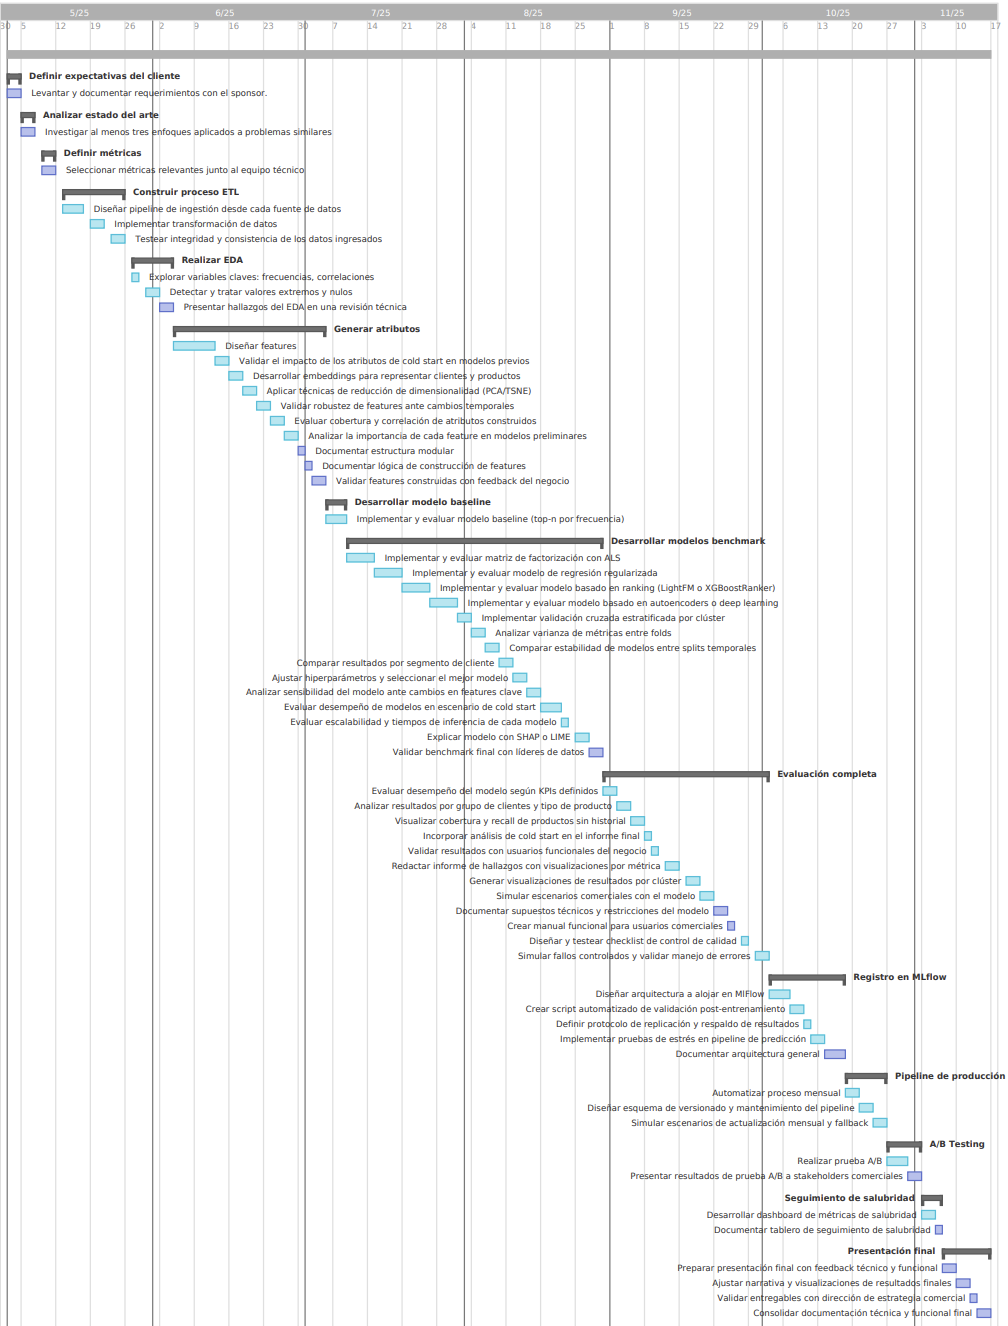
\includegraphics[height=.95\textheight]{./Figuras/Gantt.png}
\caption{Diagrama de Gantt.} 
\label{fig:diagGantt}
\end{figure}

\section{11. Planificación de Sprints}

La planificación de sprints permite organizar de manera incremental las tareas técnicas y no técnicas del proyecto. Se asegura una distribución equilibrada de la carga horaria a lo largo del desarrollo. Cada sprint representa una unidad de tiempo orientada a objetivos concretos, facilitando el seguimiento del avance y la entrega continua de resultados parciales.

Dado un compromiso de 20 horas semanales, los sprints han sido dimensionados en función de la complejidad de las tareas, sin exceder una duración estimada de 2 a 3 semanas por sprint.

\begin{longtable}{|l|l|>{\raggedright\arraybackslash}p{5cm}|l|l|l|}
\hline
\rowcolor[HTML]{C0C0C0}
Sprint & HU o fase & Tarea & Horas & Responsable & \% \\ \hline
\endfirsthead

\hline
\rowcolor[HTML]{C0C0C0}
Sprint & HU o fase & Tarea & Horas & Responsable & \% \\ \hline
\endhead

Sprint 1 & HU1 & Levantar y documentar requerimientos con el sponsor & 16 h & \authorname & 100\% \\ \hline
Sprint 2 & HU2 & Investigar y comparar enfoques aplicados a problemas similares & 17 h & \authorname & 100\% \\ \hline
Sprint 3 & HU3 & Definir y documentar métricas clave del modelo & 12 h & \authorname & 100\% \\ \hline
Sprint 4 & HU4 & Pipeline de ingestión, transformación y validación de datos & 40 h & \authorname & 0\% \\ \hline
Sprint 5 & HU5 & Análisis exploratorio y tratamiento de datos & 21 h & \authorname & 0\% \\ \hline
Sprint 6 & HU6 & Diseño de features y atributos de cold start & 30 h & \authorname & 0\% \\ \hline
Sprint 7 & HU6 & Validación y documentación de features & 41 h & \authorname & 0\% \\ \hline
Sprint 8 & HU7 & Implementar y evaluar modelo baseline & 14 h & \authorname & 0\% \\ \hline
Sprint 9 & HU8 & Modelos ALS y regresión & 40 h & \authorname & 0\% \\ \hline
Sprint 10 & HU8 & Modelos ranking y deep learning & 40 h & \authorname & 0\% \\ \hline
Sprint 11 & HU8 & Validación cruzada y sensibilidad del modelo & 40 h & \authorname & 0\% \\ \hline
Sprint 12 & HU8 & Evaluaciones de cold start y explicabilidad & 38 h & \authorname & 0\% \\ \hline
Sprint 13 & HU9 & Evaluación, visualización y documentación de resultados & 54 h & \authorname & 0\% \\ \hline
Sprint 14 & HU10 & Validación post-entrenamiento y arquitectura técnica & 41 h & \authorname & 0\% \\ \hline
Sprint 15 & HU11 & Automatización y mantenimiento del pipeline & 22 h & \authorname & 0\% \\ \hline
Sprint 16 & HU12 & Ejecutar y analizar prueba A/B & 18 h & \authorname & 0\% \\ \hline
Sprint 17 & HU13 & Desarrollo de dashboard y monitoreo de salud & 14 h & \authorname & 0\% \\ \hline
Sprint 18 & HU14 & Preparar presentación final y documentación entregable & 28 h & \authorname & 0\% \\ \hline
Sprint 19 & Redacción & Redacción de documento final & 50 h & \authorname & 0\% \\ \hline
Sprint 20 & Defensa & Preparación de exposición final & 20 h & \authorname & 0\% \\ \hline

\end{longtable}

\section{12. Normativa y cumplimiento de datos (gobernanza)}

El proyecto utiliza datos transaccionales anonimizados correspondientes a clientes B2B (kioscos y autoservicios) de una empresa del sector consumo masivo. Estos datos no contienen información personal de individuos, por lo que no están alcanzados por normativas como la Ley 25.326 de Protección de Datos Personales en Argentina en su sentido más estricto. Sin embargo, se trata de datos estratégicos cuyo tratamiento exige ciertas precauciones.

\begin{itemize}
\item Los datos han sido preprocesados y encriptados para evitar cualquier divulgación de información sensible, tanto a nivel comercial como institucional.
\item Se acordó no mencionar el nombre de la empresa en ningún entregable del proyecto, con el objetivo de preservar su confidencialidad.
\item No se requiere consentimiento explícito de usuarios, ya que no se trabaja con datos personales identificables.
\item Los datos no serán publicados ni compartidos con terceros fuera del contexto académico del proyecto.
\item Se utilizarán buenas prácticas de gobernanza de datos, tales como el acceso restringido, anonimización de variables sensibles y eliminación de los datos una vez finalizado el trabajo.
\end{itemize}

El uso de los datos es éticamente responsable y legalmente viable dentro del marco académico. El enfoque aplicado asegura el cumplimiento con los principios de confidencialidad, integridad y uso limitado, respetando los lineamientos acordados con la empresa proveedora de datos.

\section{13. Gestión de riesgos}
\label{sec:riesgos}

\subsection*{a) Identificación de riesgos y estimación de consecuencias}

Riesgo 1: despriorización del proyecto dentro de la organización
\begin{itemize}
  \item Severidad (S): 7 \\
  Si la empresa decide enfocarse en otras iniciativas, puede dificultar la obtención de validaciones y feedback funcional.
  \item Ocurrencia (O): 4 \\
  Es una posibilidad si cambian las prioridades del negocio durante los meses de desarrollo.
\end{itemize}

Riesgo 2: complejidad excesiva en la implementación del modelo de \textit{ranking} o \textit{deep learning}
\begin{itemize}
  \item Severidad (S): 7 \\
  Puede implicar replanificar entregas o reducir alcance técnico.
  \item Ocurrencia (O): 5 \\
  Probabilidad media considerando tuning, carga computacional y ajustes necesarios.
\end{itemize}

Riesgo 3: limitaciones computacionales en las instancias de entrenamiento
\begin{itemize}
  \item Severidad (S): 6 \\
  Afecta la posibilidad de experimentar con modelos complejos o validar variantes en paralelo.
  \item Ocurrencia (O): 5 \\
  Moderada, especialmente si se comparten recursos en la nube.
\end{itemize}

Riesgo 4: retrasos por revisiones internas prolongadas de entregables intermedios
\begin{itemize}
  \item Severidad (S): 6 \\
  Puede demorar iteraciones técnicas si no hay disponibilidad del equipo funcional.
  \item Ocurrencia (O): 4 \\
  Es frecuente si hay otros proyectos activos en paralelo.
\end{itemize}

Riesgo 5: continuidad laboral del alumno durante el desarrollo
\begin{itemize}
  \item Severidad (S): 8 \\
  Un corte abrupto del vínculo laboral comprometería el acceso a datos o recursos internos.
  \item Ocurrencia (O): 3 \\
  Poco probable dado el plan de carrera de la alumna, pero con alto impacto si ocurre.
\end{itemize}

\subsection*{b) Tabla de gestión de riesgos}

\begin{table}[htpb]
\centering
\begin{tabularx}{\linewidth}{@{}|X|c|c|c|c|c|c|@{}}
\hline
\rowcolor[HTML]{C0C0C0}
Riesgo & S & O & RPN & S* & O* & RPN* \\ \hline
Despriorización del proyecto & 7 & 4 & 28 & 5 & 3 & 15 \\ \hline
Complejidad en modelo ranking/deep & 7 & 5 & 35 & 6 & 3 & 18 \\ \hline
Limitaciones computacionales & 6 & 5 & 30 & 5 & 3 & 15 \\ \hline
Revisiones internas demoradas & 6 & 4 & 24 & 4 & 3 & 12 \\ \hline
Continuidad laboral del alumno & 8 & 3 & 24 & 6 & 2 & 12 \\ \hline
\end{tabularx}
\end{table}

Criterio adoptado: se aplicarán medidas de mitigación a los riesgos con RPN mayores a 25.

\subsection*{c) Plan de mitigación de los riesgos críticos}

Riesgo 1: despriorización del proyecto
\begin{itemize}
  \item Mitigación: acordar hitos intermedios con valor para la organización. Generar entregables parciales útiles aunque el proyecto no finalice completo.
  \item Severidad (S*): 5 \quad Ocurrencia (O*): 3
\end{itemize}

Riesgo 2: complejidad del modelo
\begin{itemize}
  \item Mitigación: realizar pruebas tempranas con subconjuntos y ajustar el alcance si es necesario. Priorizar modelos más interpretables en la primera etapa.
  \item Severidad (S*): 6 \quad Ocurrencia (O*): 3
\end{itemize}

Riesgo 3: limitaciones computacionales
\begin{itemize}
  \item Mitigación: reservar recursos con antelación, usar particiones y trabajar en notebooks optimizadas.
  \item Severidad (S*): 5 \quad Ocurrencia (O*): 3
\end{itemize}

\section{14. Sprint Review}
\label{sec:sprint_review}

La presente sección anticipa cómo se evaluará el cumplimiento de algunas de las funcionalidades más importantes del \textit{backlog} durante el desarrollo del proyecto. A través de esta planificación preliminar de revisiones, se definen entregables esperados, criterios de aceptación y riesgos asociados para cada historia seleccionada. Se promueve un enfoque ágil centrado en el valor entregado en cada sprint.

\begin{longtable}{|>{\raggedright\arraybackslash}m{2.3cm}|
                  >{\raggedright\arraybackslash}m{3cm}|
                  >{\raggedright\arraybackslash}m{2.5cm}|
                  >{\raggedright\arraybackslash}m{3.2cm}|
                  >{\raggedright\arraybackslash}m{2.5cm}|}
\hline
\rowcolor[HTML]{CCCCCC}
\textbf{HU seleccionada} & \textbf{Tareas asociadas} & \textbf{Entregable esperado} & \textbf{¿Cómo sabrás que está cumplida?} & \textbf{Observaciones o riesgos} \\
\hline
\endfirsthead

\hline
\rowcolor[HTML]{CCCCCC}
\textbf{HU seleccionada} & \textbf{Tareas asociadas} & \textbf{Entregable esperado} & \textbf{¿Cómo sabrás que está cumplida?} & \textbf{Observaciones o riesgos} \\
\hline
\endhead

                         & Levantar requerimientos con el sponsor &                             &                                           &                                     \\ \cline{2-2}
\multirow{-2}{=}{HU1}    & Documentar expectativas y validar con cliente & \multirow{-2}{=}{Documento de requerimientos validada} & \multirow{-2}{=}{Documento aprobado por el cliente} & \multirow{-2}{=}{Dependencia de disponibilidad del sponsor} \\
\hline
                         & Definir KPIs del modelo &                             &                                           &                                     \\ \cline{2-2}
\multirow{-2}{=}{HU3}    & Documentar fórmulas y objetivos & \multirow{-2}{=}{Documento de métricas clave} & \multirow{-2}{=}{Métricas discutidas y validadas por el equipo} & \multirow{-2}{=}{Puede requerir ajustes en etapas posteriores} \\
\hline
                         & Explorar variables clave y detectar outliers &                             &                                           &                                     \\ \cline{2-2}
\multirow{-2}{=}{HU5}    & Presentar hallazgos del EDA al equipo técnico & \multirow{-2}{=}{Notebook con EDA completo} & \multirow{-2}{=}{Análisis revisado por pares} & \multirow{-2}{=}{Retrasos si los datos son incompletos} \\
\hline
                         & Implementar modelo baseline &                             &                                           &                                     \\ \cline{2-2}
\multirow{-2}{=}{HU7}    & Evaluar con recall y coverage & \multirow{-2}{=}{Modelo base validado} & \multirow{-2}{=}{Resultados superan umbrales mínimos definidos} & \multirow{-2}{=}{Modelo poco robusto sin comparativos} \\
\hline

\end{longtable}


\section{15. Sprint Retrospective}    
\label{sec:sprint_retro}

La retrospectiva de sprint permite reflexionar sobre la forma de trabajo adoptada, incluso en una etapa inicial del proyecto. A partir del enfoque de la Estrella de la Retrospectiva, se identifican buenas prácticas, áreas de mejora y acciones concretas para optimizar la organización personal durante el desarrollo. La siguiente tabla presenta esta reflexión aplicada a distintos sprints técnicos y no técnicos.

\begin{table}[htpb]
\renewcommand{\arraystretch}{1.4}
\begin{tabular}{|>{\raggedright\arraybackslash}p{1.8cm}|
                >{\raggedright\arraybackslash}p{2.3cm}|
                >{\raggedright\arraybackslash}p{2.3cm}|
                >{\raggedright\arraybackslash}p{2.3cm}|
                >{\raggedright\arraybackslash}p{2.3cm}|
                >{\raggedright\arraybackslash}p{2.3cm}|}
\hline
\rowcolor[HTML]{CCCCCC} 
\textbf{Sprint tipo y N°} & \textbf{¿Qué hacer más?} & \textbf{¿Qué hacer menos?} & \textbf{¿Qué mantener?} & \textbf{¿Qué empezar a hacer?} & \textbf{¿Qué dejar de hacer?} \\
\hline
Sprint no técnico - 1 & Validaciones tempranas con el sponsor & Cambios sin registro & Definición clara de expectativas mínimas & Documentar criterios de aceptación & Avanzar sin confirmar requisitos \\
\hline
Sprint no técnico - 3 & Alinear definición de KPIs con el equipo & Ajustes sin justificación & Claridad en métricas clave & Registrar iteraciones de definición & Improvisar definiciones \\
\hline
Sprint técnico - 4 & Validar entradas y salidas en cada etapa & Probar sin documentación & Modularidad en scripts & Automatizar chequeos intermedios & Repetir tareas manualmente \\
\hline
Sprint técnico - 6 & Diseñar features orientadas a negocio & Duplicar atributos similares & Validaciones con el equipo & Documentar hipótesis de diseño & Trabajar sin definir targets claros \\
\hline
Sprint técnico - 9 & Comparar modelos de forma sistemática & Evaluar con pocas métricas & Trazabilidad de experimentos & Versionar datasets de entrenamiento & Ajustar sin registrar contexto \\
\hline
Sprint no técnico - 18 & Consolidar aprendizajes parciales & Reescribir sobre la marcha & Plantillas claras y homogéneas & Organizar el índice con antelación & Aplazar la escritura hasta el final \\
\hline
\end{tabular}
\end{table}

\end{document}